\documentclass{article}
\usepackage[utf8]{inputenc}
\usepackage[margin=1in]{geometry}
\usepackage{graphicx}
\usepackage{amsmath}
\setlength{\parindent}{0em}
\setlength{\parskip}{0.5em}

\title{Samantha Hassal - CTA200 2020 Assignment 2 Responses - Figures}
\date{}

\begin{document}
\begin{figure}
  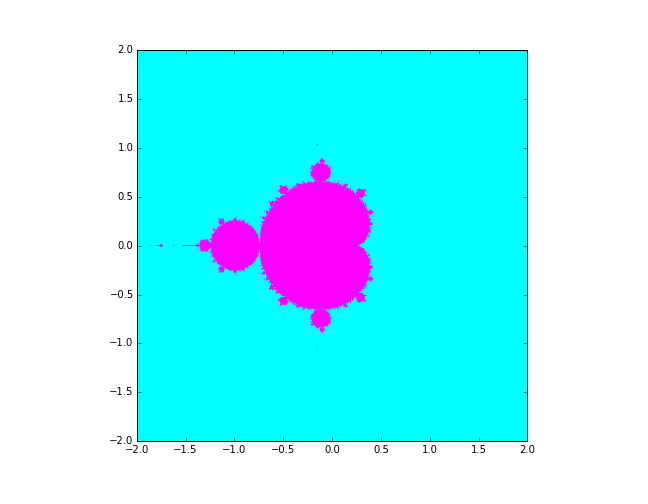
\includegraphics[width=\linewidth]{Mandel_01.png}
  \caption{The Mandelbrot set}
  \label{fig:mandelbrot1}
\end{figure}

\begin{figure}
  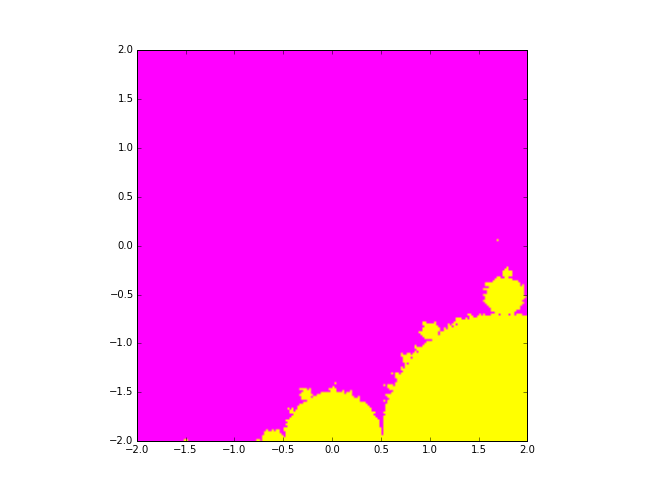
\includegraphics[width=\linewidth]{Mandel_02.png}
  \caption{A zoom-in of the Mandelbrot set}
  \label{fig:mandelbrot2}
\end{figure}

\begin{figure}
  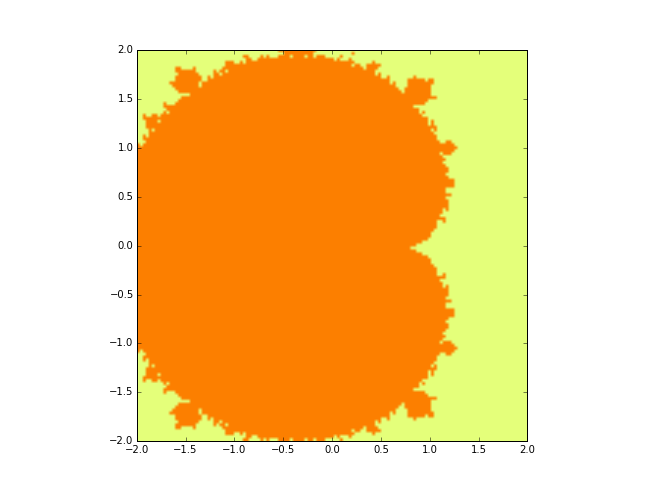
\includegraphics[width=\linewidth]{Mandel_03.png}
  \caption{Another zoom-in of the Mandelbrot set}
  \label{fig:mandelbrot3}
\end{figure}

\begin{figure}
  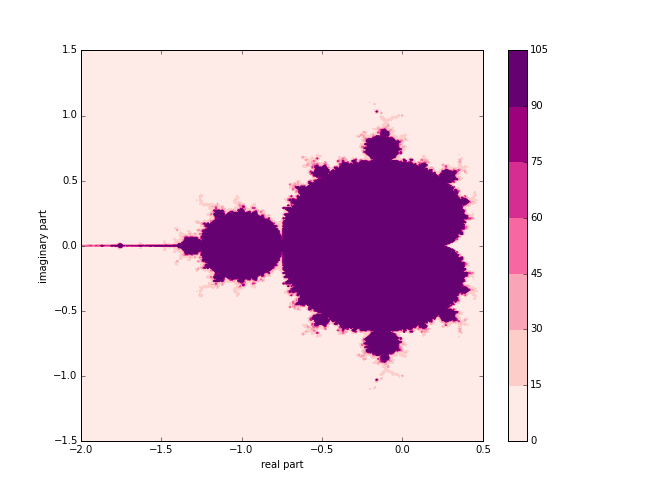
\includegraphics[width=\linewidth]{Mandel_div.png}
  \caption{The Mandelbrot set with the divergence points coloured. Colour represents the modulus at which it diverged}
  \label{fig:mandelbrot3}
\end{figure}

\begin{figure}
  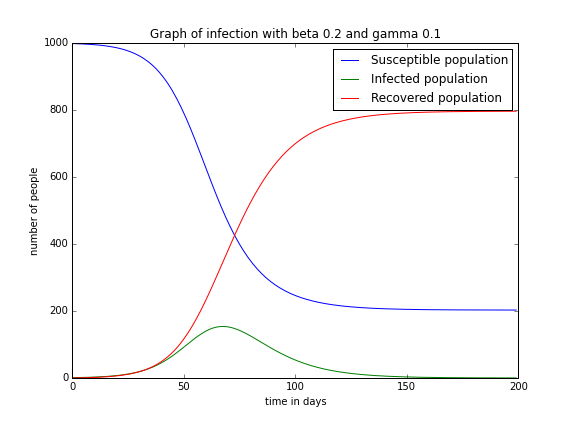
\includegraphics[width=\linewidth]{beta_greater.png}
  \caption{contact rate greater than the recovery rate}
  \label{fig:beta_greater}
\end{figure}

\begin{figure}
  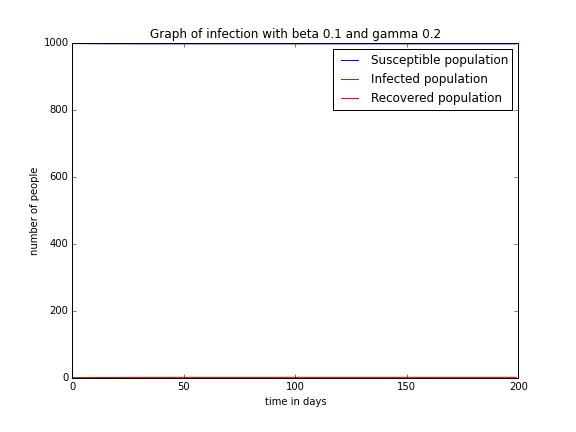
\includegraphics[width=\linewidth]{beta_less.png}
  \caption{contact rate less than the recovery rate}
  \label{fig:beta_less}
\end{figure}

\begin{figure}
  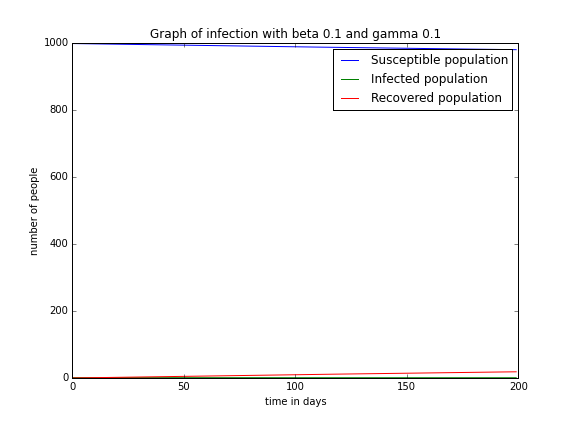
\includegraphics[width=\linewidth]{beta_gamma_equal.png}
  \caption{contact rate equals recovery rate}
  \label{fig:beta_equal_gamma}
\end{figure}

\end{document}
